\documentclass[12pt]{report}
\usepackage[spanish]{babel}
\usepackage[utf8]{inputenc}
\usepackage{graphicx}
\usepackage{verbatim}
\usepackage{listings}
\usepackage{float}
\renewcommand*\thesection{\arabic{section}}

\begin{document}
	
	\begin{center}
		\textbf{Análisis de Algoritmos, Sem: 2018-1, 3CV1, Práctica 5, 10-2017}
		\newline
	\end{center}
	
	\begin{center}
		\begin{picture}(0,0) \put(-125,-55){
			\includegraphics[width=2.7cm]{../../IPNlogo.jpg}} 
		\end{picture}
		\LARGE Escuela Superior de Cómputo.\\
		Instituto Politécnico Nacional, México.\\
		\begin{picture}(0,0) \put(160,10){
			\includegraphics[width=2.7cm]{../../logoescom.png}} 
		\end{picture}
	\end{center}
	
	\begin{center}
		\Large Práctica 5: Algoritmo de Strassen.\\
	\end{center}
	
	\begin{center}
		\textbf{Blancas Pérez Bryan Israel}\\
		orionmunecaycanica@gmail.com\\
	\end{center}
	
	
	\textbf{\large Resumen: }Implementar el algoritmo de Strassen y comparar, experimentalmente, el orden de complejidad con el algoritmo de multiplicación matricial común.\newline\\
	
	\textbf{\large Palabras Clave: } Strassen, multiplicación matricial.\\
	

	\section{Introducción}
	En esta práctica, se desea llevar a cabo la multiplicación de dos matrices, A y B. Para ello, primero se implementará el algoritmo recursivo usual de multiplicación de matrices, para obtener mediante gráficas, el orden de complejidad computacional. Después se implementará el algoritmo de Stressen y se compararán los resultados con el algoritmo usual, para poder determinar cual es mejor.\newpage
	
	
	
	\section{Conceptos Básicos}
	\textbf{Algoritmo convencional para multiplicar dos matrices.}\\
	
	El algoritmo más usual para multiplicar matrices, tiene un orden de complejidad $\theta (n^3)$. Este algoritmo se basa en la definición de multiplicación de matrices, la cual es: \newline \newline
	Sean dos matrices dadas por: \newline
	$A := a_{(ij) \ m*n} \ \ y \ \ B := b_{(ij) \ n*p} $ \newline \newline 
	Entonces la multiplicación de $A$ por $B$, es: \newline 
	$C = AB := c_{(ij) \ m*p}$ \newline \newline
	Donde cada elemento $c_{ij}$, está dado por: \newline 
	$C_{ij} \ = \ \sum_{r=1}^{n} (a_{ir}*b_{rj})$ \newline \newline
		
	\textbf{Algoritmo de Strassen.}\\
	
El Algoritmo de Strassen es un algoritmo que consiste en la multiplicación de matrices. Es más rápido que el algoritmo de multiplicación de matrices estándar, y es útil en la práctica para matrices grandes [1]. Para el algoritmo de Strassen se divide las matrices en 4 cuadrantes, y se definen las siguientes matrices:\newline
$s_{1}=(a_{1,2}-a_{2,2})(b_{2,1}+b_{2,2})$\newline
$s_{2}=(a_{1,1}+a_{2,2})(b_{1,1}+b_{2,2})$\newline
$s_{3}=(a_{1,1}-a_{2,1})(b_{1,1}+b_{1,2})$\newline
$s_{4}=(a_{1,1}+a_{1,2})b_{2,2}$\newline
$s_{5}=a_{1,1}(b_{1,2}-b_{2,2})$\newline
$s_{6}=a_{2,2}(b_{2,1}-b_{1,1})$\newline
$s_{7}=(a_{2,1}+a_{2,2})b_{1,1}$\newline
y se hacen las siguientes operaciones para la matriz resultado:\newline
$c_{1,1}=s_{1}+s_{2}-s_{4}+s_{6}$\newline
$c_{1,2}=s_{4}+s_{5}$\newline
$c_{2,1}=s_{6}+s_{7}$\newline
$c_{2,2}=s_{2}-s_{3}+s_{5}-s_{7}$\newline
Este algoritmo tiene un orden de complejidad teórico de $\theta (n^{2.8})$\newpage
		
	\section{Experimentación y Resultados}	
	\textbf{Ejercicio 1.}\\
	Implementar el algoritmo Strassen.\newline
	
	\textbf{i) Mediante gráficas, muestre que el algoritmo Strassen tiene orden de complejidad $\theta (n^{2.8})$.}\newline
	Pseudocódigo del algoritmo Strassen:
	\lstset{language=C, breaklines=true, basicstyle=\footnotesize}
	\lstset{numbers=left, numberstyle=\tiny, stepnumber=1, numbersep=10pt}
	\begin{lstlisting}
Strassen(A,B,n):
  C[n][n]
  if n==2:
    multiplicacion de matrices 2x2
  else:
    s1=stressen((a12-a22),(b21+b22),n/2)
    s2=stressen((a11+a22),(b11+b22),n/2)
    s3=stressen((a11-a21),(b11+b12),n/2)
    s4=stressen((a11+a12),b22,n/2)
    s5=stressen(a11,(b12-b22),n/2)
    s6=stressen(a22,(b21-b11),n/2)
    s7=stressen((a21+a22),b11,n/2)
    
    c11=s1+s2-s4+s6
    c12=s4+s5
    c21=s6+s7
    c22=s2-s3+s5-s7
	\end{lstlisting}
	
	El algoritmo de Strassen, utiliza el paradigma divide y vencerás para resolver el problema de multiplicación matricial.\\
	
	En la Figura 1, se puede ver la gráfica $n \ vs \ t(n)$, del algoritmo de Strassen, la función que aparece con color rojo, es $t(n)=n^{2.8}$, demostrando así, que el algoritmo de Strassen está acotado por $\theta (n^{2.8})$. \newpage
	\textbf{Gráfica del algoritmo de Strassen\\}
	\begin{figure}[H]
		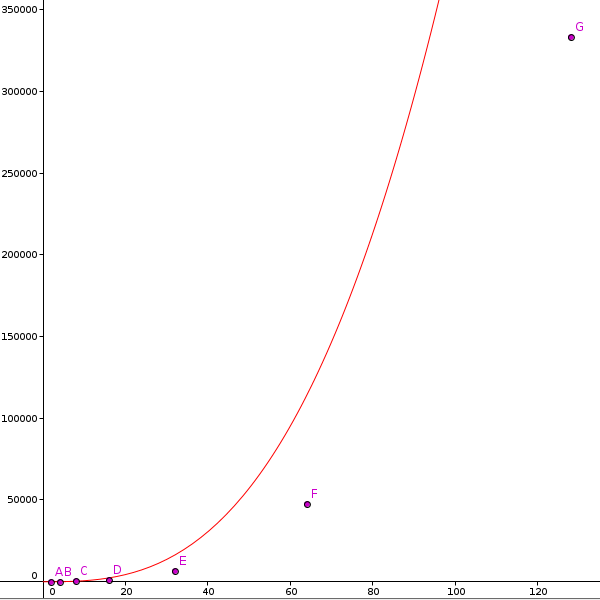
\includegraphics[width=13cm]{imagenes/1.png}
		\centering
		\caption{Algoritmo de Strassen.}
		\centering
	\end{figure}
	\newpage
			
	\textbf{ii) Para valores muy grandes de matrices compare el algoritmo de Stressen con el	producto usual de matrices (comparara la complejidad)..}\newline
		
	En la Figura 2, se puede ver la gráfica $n \ vs \ t(n)$de ambos algoritmos, el algoritmo de Strassen, aparece con puntos color rosa, y el algoritmo estándar con puntos color azul. Se aprecia que el algoritmo estándar, tiene un grado de complejidad más alto ($\theta (n^3)$), y se aprecia a partir de n=64.\newline
	
	\textbf{Gráfica de comparación de algoritmos.\\}
	\begin{figure}[H]
		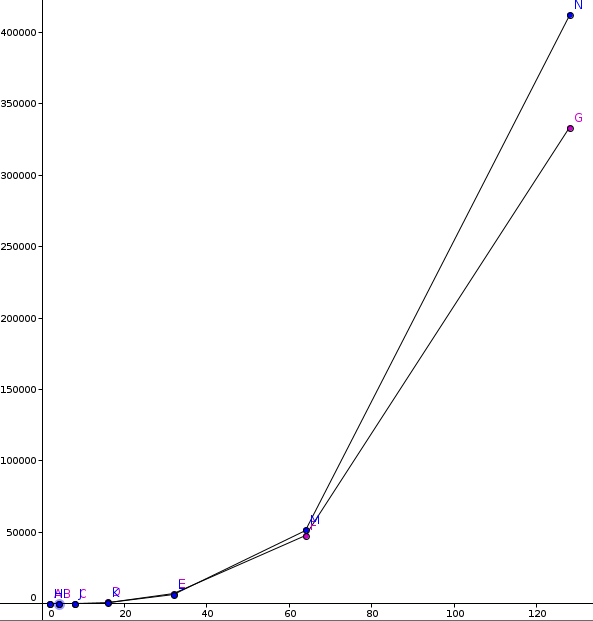
\includegraphics[width=9cm]{imagenes/2.png}
		\centering
		\caption{Comparación de algoritmos.}
		\centering
	\end{figure}
	\newpage
	
\section{Conclusiones}
Esta práctica me gusto porque representó un reto al momento de implementar el algoritmo. Tuve muchos problemas, primero, en comprender la lógica detrás del algoritmo, ya que la recursividad aplicada no era sencilla de entender. Y después, al momento de implementar el algoritmo, porque tenía que tener en cuenta el tamaño de las matrices y además, ubicar el cuadrante con el que iba a hacer las operaciones.\newline
Es increíble para mi, darme cuenta de que durante mucho tiempo se ha intentado bajar el orden de complejidad de la multiplicación de matrices, ya que nunca me había puesto a pensar en los beneficios que eso implicaría. Actualmente el algoritmo de multiplicación de matrices con menor orden de complejidad, es el algoritmo de Virginia Vassilevska Williams, con un orden de $\theta (n^{2.373})$.

\section{Bibliografía}

[1] https://es.wikipedia.org/wiki/AlgoritmodeStrassen
	
\end{document}